\section{背景}
\label{sec:background}

% 翻译完成

% \egg builds on \egraphs and equality saturation.
%   This section describes those techniques and
%   presents the challenges that \egg addresses.
\egg 建立在 \egraphs 和 等式饱和 的基础上。
  本节描述了这些技术,并介绍了 \egg 所要解决的挑战。

% % Many problems in program optimization, theorem proving,
% %   and other domains have a similar shape:
% % given an input expression, search for a ``better'' equivalent
% %   expression.
% % This paper puts forward the case that, with our proposed advances, equality
% %   saturation is now the right tool for the job in many cases like
% %   these.

% % We will work through an extended example around optimizing
% %   the expression
% %   $(a \times 2) / 2$
% %   and discover the benefits of \egraphs and equality saturation,
% %   current limitations of using and implementing this approach,
% %   and how \egg addresses those limitations.

% \subsection{\Egraphs}
\subsection{\Egraphs (e 图)}
\label{sec:egraphs}

% An \textit{\egraph} is a data structure that stores a set of terms and a
%   congruence relation over those terms.
% Originally developed for and still used in the
%   heart of theorem provers~\cite{nelson, simplify, z3},
%   \egraphs have also been used to power a program optimization technique
%   called \textit{equality saturation}~%
%   \cite{denali, eqsat, eqsat-llvm, szalinski, yogo-pldi20, spores, herbie}.
一个 \textit{\egraph} 是一个数据结构,
  它存储了一组项(term)和这些项上的一个同义关系。
它最初是为定理证明器开发的,现在仍然被用于定理证明器的核心~\cite{nelson, simplify, z3},
  \egraphs 也被用来支持一种程序优化技术称为 \textit{等式饱和(equality saturation)}~。
  \cite{denali, eqsat, eqsat-llvm, szalinski, yogo-pldi20, spores, herbie}.。
  
% \subsubsection{Definitions}
\subsubsection{定义}

% \begin{figure}
%   \centering
%   \begin{align*}
%      \text{function symbols} \quad & f,g                                   \\[-0.2em]
%      \text{\eclass ids} \quad & a,b & \text{opaque identifiers}            \\[-0.2em]
%      \text{terms}     \quad & t  ::= f \mid f(t_1, \ldots, t_m) & m \geq 1 \\[-0.2em]
%      \text{\enodes}   \quad & n  ::= f \mid f(a_1, \ldots, a_m) & m \geq 1 \\[-0.2em]
%      \text{\eclasses} \quad & c  ::= \{ n_1, \ldots, n_m \}     & m \geq 1
%   \end{align*}
%   \caption{
%     Syntax and metavariables for the components of an \egraph.
%     Function symbols may stand alone as constant \enodes and terms.
%     An \eclass id is an opaque identifier that can be compared for equality with $=$.
%   }
%   \label{fig:syntax}
% \end{figure}
\begin{figure}
  \centering
  \begin{align*}
     \text{函数符号} \quad & f,g                                   \\[-0.2em]
     \text{\eclass ids} \quad & a,b & \text{opaque identifiers}            \\[-0.2em]
     \text{terms}     \quad & t  ::= f \mid f(t_1, \ldots, t_m) & m \geq 1 \\[-0.2em]
     \text{\enodes}   \quad & n  ::= f \mid f(a_1, \ldots, a_m) & m \geq 1 \\[-0.2em]
     \text{\eclasses} \quad & c  ::= \{ n_1, \ldots, n_m \}     & m \geq 1
  \end{align*}
  \caption{
    语法和元变量为一个 \egraph 的组成部分。函数符号可以作为常数 \enodes 和项单独存在。
    一个\eclass id 是一个不透明的标识符,可以用 $=$ 来比较是否相等。
  }
  \label{fig:syntax}
\end{figure}


% Intuitively,
%   an \egraph is a set of equivalence classes (\textit{\eclasses}).
% Each \eclass is a set of \textit{\enodes} representing equivalent terms from a given language,
%   and an \enode is a function symbol paired with a list of children \eclasses.
% More precisely:

直观地,一个 \egraph 是一组等价类(\textit{\eclasses})。
每个 \eclass 是一组代表特定语言中等价项的 \textit{\enodes} 。
  而一个 \enode 是一个函数符号与一个子 \eclasses 列表的配对。
更确切地:

% \begin{definition}[Definition of \Egraph]
%   \label{def:egraph}

%   Given the definitions and syntax in \autoref{fig:syntax},
%   an \textit{\egraph} is a tuple $(U, M, H)$ where:
%   \begin{itemize}
%     \item
%     A union-find data structure~\cite{unionfind} $U$
%       stores an equivalence relation (denoted with $\equivid$)
%       over \eclass ids.

%     \item
%     The \textit{\eclass map} $M$ maps \eclass ids to \eclasses.
%     All equivalent \eclass ids map to the same \eclass, i.e.,
%       $a \equivid b$ iff $M[a]$ is the same set as $M[b]$.
%     An \eclass id $a$ is said to \textit{refer to} the \eclass $M[\find(a)]$.

%     \item The \textit{hashcons}\footnote{
%       We use the term \textit{hashcons} to evoke the memoization technique,
%       since both avoid creating new duplicates of existing objects.
%     }
%     $H$ is a map from \enodes to \eclass ids.
%   \end{itemize}

%   % An \textit{\eclass} is a set of \enodes.
%   % An \textit{\enode} $f(a_{1}, ..., a_{n})$ is
%   %   a function symbol $f$ from the given language
%   %   and a (potentially empty) list of \eclass ids.

%   Note that an e-class has an identity
%    (its canonical \eclass id),
%    but an \enode does not.\footnote{
%     Our definition of an \egraph reflects \egg's design
%       and therefore differs with some other \egraph definitions and implementations.
%     In particular, making e-classes but not e-nodes identifiable is unique to
%       our definition.
%   }
%   We use \eclass id $a$ and the \eclass $M[\find(a)]$ synonymously when clear from the context.
% 
% \end{definition}
\begin{definition}[单个 \Egraph 的定义]
  \label{def:egraph}

  给定 \autoref{fig:syntax} 中的定义与语法,
  一个 \textit{\egraph} 是一个元组(tuple) $(U, M, H)$ ,其中:
  \begin{itemize}
    \item
    一个并查集(union-find ~\cite{unionfind}) $U$
      存储了一个 \eclass id 等价关系(用 $\equivid$ 表示)。% ?ids
      
    \item
    \textit{\eclass map} $M$ 将 \eclass id 映射到 \eclasses。
    所有等价的 \eclass id 都映射到相同的 e-class,即,
    $a \equivid b$ 当且仅当 $M[a]$ 与 $M[b]$ 是同一个集合。
    一个 \eclass id $a$ 被称为 
    \textit{refer to} \eclass $M[\find(a)]$.  %?is said to \textit{refer to} 

    \item \textit{hashcons}\footnote{
      我们使用术语 \textit{hashcons} (哈希康)来引入记忆化技术,
      因为两者都可以避免创建现有对象的新副本。 % 两者 ?
    }
    $H$ 是 \enodes 到 \eclass id 的映射(map).
  \end{itemize}
   请注意,一个 e-class 有一个 ID (它的规范(canonical) \eclass id)。
   但一个 \enode 没有。\footnote{
    我们对 \egraph 的定义反映了 \egg 的设计,因此不同于其他一些 \egraph 的定义和实现。
    我们的定义的特别之处是使用可识别的 e-classes 而不是 e-nodes。
  }
  无歧义时,我们使用 \eclass id $a$ 指代 \eclass $M[\find(a)]$ 。% 同义于

\end{definition}

% \begin{definition}[Canonicalization]
%     An \egraph's union-find $U$ provides a \find operation that canonicalizes \eclass ids
%       such that ${\find(U, a) = \find(U, b)}$ iff ${a \equivid b}$.
%     We omit the first argument of \find where clear from context.
%     \begin{itemize}
%       \item An \eclass id $a$ is canonical iff $\find(a) = a$.
%       \item \raggedright
%             An \enode $n$ is canonical iff $n = \texttt{canonicalize}(n)$,
%             where ${\texttt{canonicalize}(f(a_{1}, a_{2}, ...)) = f(\find(a_{1}), \find(a_{2}), ...)}$.
%     \end{itemize}
% \end{definition}
\begin{definition}[规范化]
    一个 \egraph 的并查集 $U$ 提供一个 \find 操作, 能规范化(canonicalizes) \eclass id
      以便 ${\find(U, a) = \find(U, b)}$ 当且仅当 ${a \equivid b}$。 % ? canonicalizes
    无歧义时,我们忽略 \find 的第一个参数。
    \begin{itemize}
      \item 一个 \eclass id $a$ 是规范的 当且仅当 $\find(a) = a$.
      \item \raggedright
            一个 \enode $n$ 是规范的 当且仅当 $n = \texttt{canonicalize}(n)$,
            此时  %?where
            ${\texttt{canonicalize}(f(a_{1}, a_{2}, ...)) = f(\find(a_{1}), \find(a_{2}), ...)}$. 
    \end{itemize}
\end{definition}

% \begin{definition}[Representation of Terms]
%   An \egraph, \eclass, or \enode is said to \textit{represent} a term $t$ if $t$ can be
%     ``found'' within it. Representation is defined recursively:
%   \begin{itemize}
%     \item An \egraph represents a term if any of its \eclasses do.
%     \item An \eclass $c$ represents a term if any \enode $n \in c$ does.
%     \item An \enode $f(a_{1}, a_{2}, ...)$ represents a term $f(t_{1}, t_{2}, ...)$
%           if they have the same function symbol $f$
%           and \eclass $M[a_{i}]$ represents term $t_{i}$.
%   \end{itemize}

%   When each \eclass is a singleton (containing only one \enode),
%     an \egraph is essentially a term graph with sharing.
%   \autoref{fig:egraph-rewrite1} shows an \egraph that represents the
%     expression $(a \times 2) / 2$.
% \end{definition}
\begin{definition}[项(term)的表示]
  一个 \egraph、\eclass 或 \enode 被称为 \textit{表示} 一个项 $t$,
    如果 $t$ 可以在其中被 ``发现''。表示的方法是递归定义的:
  \begin{itemize}
    \item 一个 \egraph 表示一个项如果它的每一个 \eclasses 也是这样的。
    \item 一个 \eclass $c$ 表示一个项如果每一个 \enode $n \in c$ 也是这样的。
    \item 一个 \enode $f(a_{1}, a_{2}, ...)$ 表示一个项 $f(t_{1}, t_{2}, ...)$
          如果它们有一样的的函数符 $f$ 并且 \eclass $M[a_{i}]$ 表示项 $t_{i}$.
  \end{itemize}

  当每个 \eclass 是一个单子(singleton,只包含一个 \enode),一个 \egraph 本质上是一个共享的项图(term graph)。
  \autoref{fig:egraph-rewrite1} 显示了一个代表表达式 $(a\times 2) / 2$ 的 \egraph。
\end{definition}

% \begin{definition}[Equivalence]
%   An \egraph defines three equivalence relations.
%   \begin{itemize}
%     \item Over \eclass ids: $a \equivid b$ iff $\find(a) = \find(b)$.
%     \item Over \enodes: $n_{1} \equivnode n_{2}$ iff \enodes $n_{1}, n_{2}$ are in the same \eclass, 
%           i.e., $\exists a.\ n_{1}, n_{2} \in M[a]$.
%     \item Over terms: $t_{1} \equivterm t_{2}$ iff terms $t_{1}, t_{2}$ are represented in the same \eclass.
%   \end{itemize}

%   We use $\equiv$ without the subscript when the relation is clear from context.
% \end{definition}
\begin{definition}[等价,Equivalence]
  一个 \egraph 定义了三个等价关系。
  \begin{itemize} % Over的翻译?
    \item 对于 \eclass id: $a \equivid b$ 当且仅当 $\find(a) = \find(b)$.
    \item 对于 \enodes: $n_{1} \equivnode n_{2}$ 当且仅当 \enodes $n_{1}, n_{2}$ 在同样的 \eclass 里, 
          也就是说, $\exists a.\ n_{1}, n_{2} \in M[a]$.
    \item 对于 terms: $t_{1} \equivterm t_{2}$ 当且仅当 terms $t_{1}, t_{2}$ 以相同的 \eclass 表示。
  \end{itemize}

  无歧义时,我们使用无下标的 $\equiv$ 。
\end{definition}

% \begin{definition}[Congruence]
%   For a given \egraph, let $\cong$ denote a congruence relation over \enodes such that
%   ${f(a_{1}, a_{2}, ...) \cong f(b_{1}, b_{2}, ...)}$ iff $a_{i} \equivid b_{i}$.
%   Let $\cong^{*}$ denote the congruence closure of $\equivnode$,
%    i.e., the smallest superset of $\equivnode$ that is also a superset of $\cong$.
%   Note that there may be two \enodes such that
%     $n_{1} \cong^{*} n_{2}$ but
%     $n_{1} \not\cong n_{2}$ and
%     $n_{1} \not\equivnode n_{2}$.
%   The relation $\cong$ only represents a single step of congruence;
%   more than one step may be required to compute the congruence closure.
% \end{definition}
\begin{definition}[同余,Congruence] 
  对于一个给定的 \egraph ,让 $\cong$ 表示在 \enodes 上的一个全等关系,以便
  ${f(a_{1}, a_{2}, ...) \cong f(b_{1}, b_{2}, ...)}$ 当且仅当 $a_{i} \equivid b_{i}$。
  让 $\cong^{*}$ 表示 $\equivnode$ 的全等闭包(congruence closure)。
    % congruence closure?参考:https://zhuanlan.zhihu.com/p/90143262
   即 $\equivnode$ 的最小的超集,同时也是 $\cong$ 的超集。
  请注意,可能有两个 \enodes ,以便
    $n_{1} \cong^{*} n_{2}$ 但是
    $n_{1} \not\cong n_{2}$ 且
    $n_{1} \not\equivnode n_{2}$.
  关系 $\cong$ 只代表一个单步的同余,计算全等闭包可能需要一个以上的步骤。
  
\end{definition}

% \subsubsection{\Egraph Invariants}
\subsubsection{\Egraph 不变量}
\label{sec:invariants}

% The \egraph must maintain invariants in order to
%   correctly and efficiently implement the operations given in \autoref{sec:interface}.
% This section only defines the invariants,
%   discussion of how they are maintained is deferred to \autoref{sec:rebuild}.
% These are collectively referred to as the \textit{e-graph invariants}.
\egraph 必须保持不变性,以便正确有效地实现 \autoref{sec:interface} 中的操作。
本节只定义了不变量(invariants),
  关于如何维护这些不变量的讨论推迟到 \autoref{sec:rebuild} 中。
这些被统称为 \textit{\Egraph 不变量(e-graph invariants)}。

% \begin{definition}[The Congruence Invariant]
%   \label{def:cong-inv}
%   The equivalence relation over \enodes must be closed over congruence,
%     i.e., $(\equivnode) = (\cong^{*})$.
%   The \egraph must ensure that congruent \enodes are in the same \eclass.
%   Since identical \enodes are trivially congruent,
%    this implies that an \enode must be uniquely contained in a single \eclass.
% \end{definition}
\begin{definition}[同余不变量(Congruence Invariant)]
  \label{def:cong-inv}
   \enodes 上的等价关系必须是闭合的同余关系,也就是说,$(\equivnode) = (\cong^{*})$。
  该 \egraph 必须确保同余的 \enodes 是在同一个 \eclass 中。
  由于相同的 \enodes 是 平凡的同余的(trivially congruent)。
   这意味着一个 \enode 必须唯一地包含在一个单一的 \eclass 中。
\end{definition}

% \begin{definition}[The Hashcons Invariant]
%   \label{def:hash-inv}
%   The hashcons $H$ must map all canonical \enodes to their \eclass ids.
%   In other words:
%   $$ \enode\ n \in M[a] \iff H[\texttt{canonicalize}(n)] = \find(a) $$
%  % for each pair $(n, a) \in H$, \enode $n$ must be canonical and $n \in M[a]$.

%   If the hashcons invariant holds, then a procedure $\texttt{lookup}$
%     can quickly find which \eclass (if any) has an \enode congruent to a given \enode $n$:
%   $\texttt{lookup}(n) = H[\texttt{canonicalize}(n)]$.
% \end{definition}
\begin{definition}[哈希康不变量(Hashcons Invariant)] % ?哈希康 Hashcons Invariant
  \label{def:hash-inv}
  哈希康 $H$ 必须将所有规范 \enodes 映射到其 \eclass id。换言之:
  $$ \enode\ n \in M[a] \iff H[\texttt{canonicalize}(n)] = \find(a) $$
 % % for each pair $(n, a) \in H$, \enode $n$ must be canonical and $n \in M[a]$.

  如果哈希康不变量成立,那么一个程序 $\texttt{lookup}$ 
    就可以快速找到哪个 \eclass (如果有的话)有一个与给定的 \enode $n$ 同余的 \enode :
  $\texttt{lookup}(n) = H[\texttt{canonicalize}(n)]$。 \footnote{
     【译注】\; \texttt{canonicalize} :规范化转换
    }
\end{definition}

% 原文注释 begin -------------
%   \Remy{How can add violate deduplication?}
% Traditionally, \egraphs employ two techniques to maintain the invariants on
%   every call to \texttt{add} or \texttt{merge}.

% As \eclasses grow, the \egraph represents exponentially (or even infinitely) many terms,
%   one for every choice of representative \enode for each \eclass.
% The \egraph in \autoref{fig:egraph-rewrite-before} is essentially an AST with
%   sharing, since each \eclass is a singleton.

% \Egraphs are manipulated by two main operations:
%   adding new \enodes (into new \eclasses)
%   and merging \eclasses (sometimes called \textit{asserting} equivalences).
% \Chandra{since this is POPL, I feel that we might be expected to
% write invariants like the following a bit more formally?}
% These operations maintain two important invariants, which we will call the
%   \textit{\egraph invariants}:
% \begin{enumerate}
%   \item Deduplication:
%     The \egraph must not contain two \enodes with the same operator and
%     equivalent children.
%     \Leo{clarify dedup; distinguish identical and equivalent}
%     \Leo{this doesn't necessarity hold in modern \egraphs}
%   \item Congruence:
%     The equivalence relation on terms must also be a congruence relation, i.e.
%     if $a = b$ then $f(a) = f(b)$.
% \end{enumerate}

% Both operations can violate the two \egraph's congruence invariant.

% Deduplication is typically maintained by \textit{hashconsing}, or memoizing,
%   the add operation.
% If the user tries to add an \enode that is already represented in the \egraph,
%   the \egraph should simply return the \eclass representing the \enode instead of
%   inserting the \enode.
% Congruence is traditionally maintained by keeping a list of
%   \textit{parent pointers} for each \eclass that stores which \enodes have that
%   \eclass as children.
% On the merge operation, the parents of the merged classes must be checked to see
%   if any pairs of them became equivalent, proceeding recursively until no
%   additional equivalences are found.
% 原文注释 end -------------

% \begin{figure}
%   \begin{subfigure}[t]{0.175\linewidth}
%     \centering
%     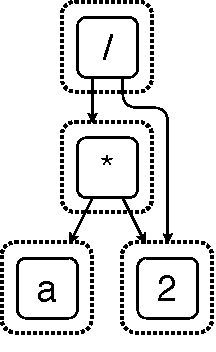
\includegraphics[height=30mm]{overview1.pdf}
%     \caption{Initial \egraph contains ${(a \times 2) / 2}$.}
%     \label{fig:egraph-rewrite1}
%   \end{subfigure}
%   \hfill
%   \begin{subfigure}[t]{0.23\linewidth}
%     \centering
%     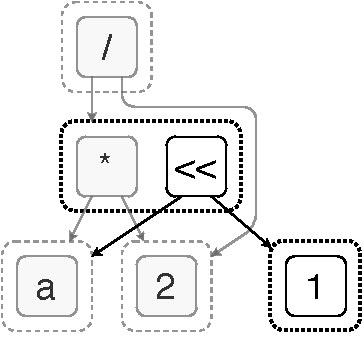
\includegraphics[height=30mm]{overview2.pdf}
%     \caption{
%       After applying rewrite ${x \times 2 \to x \ll 1}$.
%     }
%     \label{fig:egraph-rewrite2}
%   \end{subfigure}
%   \hfill
%   \begin{subfigure}[t]{0.23\linewidth}
%     \centering
%     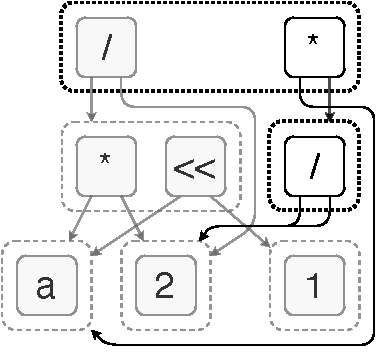
\includegraphics[height=30mm]{overview3.pdf}
%     \caption{
%       After applying rewrite ${(x \times y) / z \to x \times (y / z)}$.
%     }
%     \label{fig:egraph-rewrite3}
%   \end{subfigure}
%   \hfill
%   \begin{subfigure}[t]{0.24\linewidth}
%     \centering
%     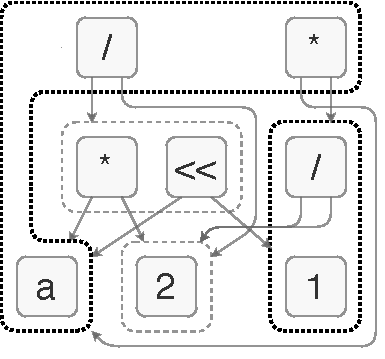
\includegraphics[height=30mm]{overview4.pdf}
%     \caption{
%       After applying rewrites ${x / x \to 1}$ and ${1 \times x \to x}$.
%     }
%     \label{fig:egraph-rewrite4}
%   \end{subfigure}
%   \caption{
%     An \egraph consists of \eclasses (dashed boxes) containing
%       equivalent \enodes (solid boxes).
%     Edges connect \enodes to their child \eclasses.
%     Additions and modifications are emphasized in black.
%     Applying rewrites to an \egraph adds new \enodes and edges,
%       but nothing is removed.
%     Expressions added by rewrites are merged with the matched \eclass.
%     In \autoref{fig:egraph-rewrite4}, the rewrites do not add any new nodes,
%       only merge \eclasses.
%     The resulting \egraph has a cycle,
%       representing infinitely many expressions:
%       $a$, $a \times 1$, $a \times 1 \times 1$, and so on.
%   }
%   \label{fig:egraph-rewrite}
% \end{figure}
\begin{figure}
  \begin{subfigure}[t]{0.175\linewidth}
    \centering
    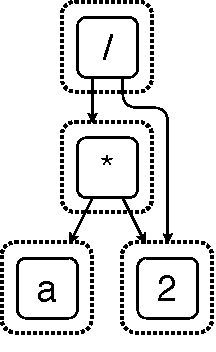
\includegraphics[height=30mm]{overview1.pdf}
    \caption{初始化包含\, ${(a \times 2) / 2}$ \,的\, \egraph}
    \label{fig:egraph-rewrite1}
  \end{subfigure}
  \hfill
  \begin{subfigure}[t]{0.23\linewidth}
    \centering
    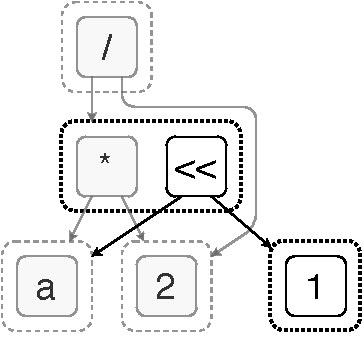
\includegraphics[height=30mm]{overview2.pdf}
    \caption{
      施加重写规则\, ${x \times 2 \to x \ll 1}$
    }
    \label{fig:egraph-rewrite2}
  \end{subfigure}
  \hfill
  \begin{subfigure}[t]{0.23\linewidth}
    \centering
    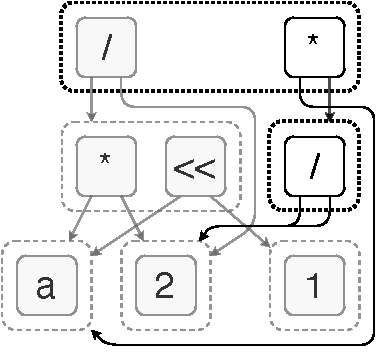
\includegraphics[height=30mm]{overview3.pdf}
    \caption{
      施加重写规则\, ${(x \times y) / z \to x \times (y / z)}$
    }
    \label{fig:egraph-rewrite3}
  \end{subfigure}
  \hfill
  \begin{subfigure}[t]{0.24\linewidth}
    \centering
    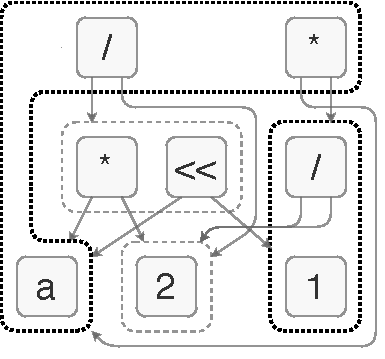
\includegraphics[height=30mm]{overview4.pdf}
    \caption{
      施加重写规则\, ${x / x \to 1}$ 和 ${1 \times x \to x}$
    }
    \label{fig:egraph-rewrite4}
  \end{subfigure}
  \caption{
    一张 \egraph 由包含等价的 \enodes(实心框)的 \eclasses (虚线框)组成。
    连接线连结 \enodes 到它们的 \eclasses 。
    加黑之处是增加和修改的部分。
    将重写应用于一个 \egraph 会增加新的 \enodes 和边线。但没有删除任何东西。
    通过改写增加的表达式会与匹配的 \eclass 合并。
    在 \autoref{fig:egraph-rewrite4} 中,改写不增加任何新节点,只是合并 \eclass。
      由此产生的 \egraph 有一个循环,代表无限多的表达式:
      $a$, $a \times 1$, $a \times 1 \times 1$, 以此类推。
  }
  \label{fig:egraph-rewrite}
\end{figure}


% \subsubsection{Interface and Rewriting}
\subsubsection{接口和重写}
\label{sec:interface}

% \Egraphs bear many similarities to the classic union-find data
%   structure that they employ internally,
%   and they inherit much of the terminology.
% \Egraphs provide two main low-level mutating operations:
\Egraphs 与经典的数据结构并查集有许多相似之处,它在内部采用了这种结构,继承了很多术语。
\Egraphs 提供了两个主要的低级变异操作:

% \begin{itemize}
%     \item \texttt{add} takes an \enode $n$ and:
%     \begin{itemize}
%         \item if $\texttt{lookup}(n) = a$, return $a$;
%         \item if $\texttt{lookup}(n) = \emptyset$,
%               then set $M[a] = \{ n \}$ and return the id $a$.
%     \end{itemize}
%     \item \texttt{merge} (sometimes called \texttt{assert} or \texttt{union})
%     takes two \eclass ids $a$ and $b$,
%     unions them in the union-find $U$,
%     and combines the \eclasses by setting both $M[a]$ and $M[b]$ to $M[a] \cup M[b]$.
% \end{itemize}
\begin{itemize}
    \item \texttt{add} 接受一个 \enode $n$ 进行:
    \begin{itemize}
        \item 如果 $\texttt{lookup}(n) = a$, 返回 $a$;
        \item 如果 $\texttt{lookup}(n) = \emptyset$,
              则设置 $M[a] = \{ n \}$ 并且返回 id $a$.
    \end{itemize}
    \item \texttt{merge} (有些时候称为 \texttt{assert} 或 \texttt{union})
    接受两个 \eclass id :$a$ 和 $b$,
    在并查集 $U$ 中合并它们, 
    然后通过设置 $M[a]$ 与 $M[b]$ 到 $M[a] \cup M[b]$ 拼合 \eclasses 。 % ?combines 拼合
\end{itemize}

% Both of these operations must take additional steps to maintain the congruence
%   invariant.
% Invariant maintenance is discussed in \autoref{sec:rebuilding}.
这两种操作都必须采取额外的步骤来维持同余的不变量。
不变量维护将在 \autoref{sec:rebuilding} 中讨论。

% \Egraphs also offers operations for querying the data structure.
\Egraphs 还提供了查询数据结构的操作:

% \begin{itemize}
%     \item \texttt{find} canonicalizes \eclass ids using the union-find $U$ as described in definition \ref{def:egraph}.
%     \item \texttt{ematch} performs the
%           \textit{e-matching}~\cite{simplify, ematching}
%           procedure for finding patterns in the \egraph.
%           \texttt{ematch} takes a pattern term $p$ with variable placeholders
%           and returns a list of tuples $(\sigma, c)$ where $\sigma$ is a substitution of
%           variables to \eclass ids such that $p[\sigma]$ is represented in \eclass $c$.
% \end{itemize}
\begin{itemize}
    \item \texttt{find} 使用并查集 $U$ 来进行规范化 \eclass id,如定义 \ref{def:egraph} 所述。
    \item \texttt{ematch} 执行在 \egraph 中查找模式的 
          \textit{e-matching}~\cite{simplify, ematching} 过程。 
          \texttt{ematch} 接受一个具有变量占位符的模式项 $p$ 并返回一个元组列表 $(\sigma, c)$,
          其中 $\sigma$ 是变量到 \eclass id 的替换,使得 $p[\sigma]$ 能在 \eclass $c$ 中表示。
            % ? 
\end{itemize}


% These can be composed to perform rewriting over the
%   \egraph.
% To apply a rewrite $\ell \to r$ to an \egraph,
%   \texttt{ematch}
%   finds tuples $(\sigma, c)$ where \eclass $c$ represents $\ell[\sigma]$.
% Then, for each tuple,
%   \mbox{\texttt{merge($c$, add($r[\sigma]$))}} adds $r[\sigma]$ to the \egraph
%   and unifies it with the matching \eclass c.
这些可以组合起来对 \egraph 执行重写。
要在 \egraph 上应用重写 $\ell \to r$ ,
  \texttt{ematch} 会找到元组 $(\sigma, c)$ ,其中 \eclass $c$ 表示 $\ell[\sigma]$ 。
然后,对于每个元组,
  \mbox{\texttt{merge($c$, add($r[\sigma]$))}} 将 $r[\sigma]$ 添加到 \egraph 中,
  并使其与匹配的 \eclass c 统一。


% \autoref{fig:egraph-rewrite} shows an \egraph undergoing a series of rewrites.
% Note how the process is only additive; the initial term $(a \times 2) / 2$ is
%   still represented in the \egraph.
% Rewriting in an \egraph can also saturate, meaning the \egraph has
%   learned every possible equivalence derivable from the given rewrites.
% % This not only solves the phase ordering problem, but also handles rules like
% %   commutativity that can be troublesome to a conventional rewrite system.
% If the user tried to apply $x \times y \to y \times x$ to an \egraph twice,
%   the second time would add no additional \enodes and perform no new merges;
%   the \egraph can detect this and stop applying that rule.
\autoref{fig:egraph-rewrite} 展示了一个经历了一系列重写的 \egraph。
注意这个过程只是增加性的;初始项 $(a \times 2) / 2$ 仍然在 \egraph 中表示。
在 \egraph 中重写也可以饱和,这意味着 \egraph 已经学会了给定重写可以推出的所有等价关系。
% 这不仅解决了阶段顺序问题,还能处理像交换律这样的规则,这对于传统重写系统来说可能有困难。
如果用户试图将 $x \times y \to y \times x$ 应用于 \egraph 两次,
  第二次将不会添加额外的 \enodes 并不会进行新的合并;\egraph 可以检测到这一点并停止应用该规则。

\subsection{等式饱和(Equality Saturation)}
\label{sec:eqsat}

% Term rewriting~\cite{nachum-rewrites} is a time-tested approach
%   for equational reasoning in
%   program optimization~\cite{eqsat, denali},
%   theorem proving~\cite{simplify, z3},
%   and program transformation~\cite{graphs}.
% In this setting, a tool repeatedly chooses one of a set of axiomatic rewrites,
%   searches for matches of the left-hand pattern in the given
%   expression, and replaces matching instances with the substituted
%   right-hand side.
项重写 ~\cite{nachum-rewrites} 是一种久经考验的方法,
  它针对于程序综合~\cite{eqsat, denali}、
  定理证明~\cite{simplify, z3}、
  程序转换~\cite{graphs},
  中的等式推理
在这种情况下,一个工具重复选择一组公理改写中的一个。
  在给定的表达式中搜索与左式相匹配的表达式,并将匹配的实例替换为被替换的右式。

% Term rewriting is typically destructive and ``forgets'' the matched
%   left-hand side.
% Consider applying a simple strength reduction rewrite:
%   ${ (a \times 2) / 2 \to (a \ll 1) / 2 }$.
% The new term carries no
%   information about the initial term.
% Applying strength reduction at this point prevents us from canceling out $2/2$.
% In the compilers community, this classically tricky question of when to apply
%   which rewrite is called the \textit{phase ordering} problem.
项重写通常是破坏性的并且“忘记”了匹配的左式。
考虑应用一个简单的降低计算量(strength reduction)重写:
  ${ (a \times 2) / 2 \to (a \ll 1) / 2 }$。
新项不带有初始项的信息。在此之前应用降低计算量重写阻止我们消除 $2/2$。
在编译器社群中,这个关于何时应用哪个重写的问题被称为\textit{编译优化选择(phase ordering)}问题。


% One solution to the phase ordering problem would simply apply all
%   rewrites simultaneously, keeping track of every expression seen.
% This eliminates the problem of choosing the right rule, but
%   a naive implementation would require space exponential in the number
%   of given rewrites.
% \textit{Equality saturation}~\cite{eqsat, eqsat-llvm} is a technique to do this
%   rewriting efficiently using an \egraph.
解决编译优化选择问题的一种方法是同时应用所有重写,并跟踪每个表达式。
这消除了选择正确规则的问题,但是简单实现需要给定重写数量的指数级空间。
\textit{等式饱和(equality saturation)}~\cite{eqsat, eqsat-llvm} 是一种使用 \egraph 有效地进行此重写的技术。

% \begin{figure}
%   \begin{minipage}{0.48\linewidth}
%     \centering
%     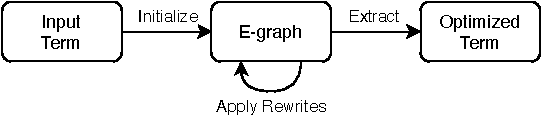
\includegraphics[width=0.9\linewidth]{eqsat}
%   \end{minipage}
%   \hfill
%   \begin{minipage}{0.46\linewidth}
%   \begin{lstlisting}[language=Python, gobble=4, numbers=left, basicstyle=\scriptsize\ttfamily]
%     def equality_saturation(expr, rewrites):
%       egraph = initial_egraph(expr)

%       while not egraph.is_saturated_or_timeout():

%         for rw in rewrites:
%           for (subst, eclass) in egraph.ematch(rw.lhs):
%             eclass2 = egraph.add(rw.rhs.subst(subst))
%             egraph.merge(eclass, eclass2)

%       return egraph.extract_best()
%   \end{lstlisting}
%   \end{minipage}
%   \caption{
%     Box diagram and pseudocode for equality saturation.
%     Traditionally, equality saturation maintains the \egraph data structure
%       invariants throughout the algorithm.
%   }
%   \label{fig:eq-sat-bg}
% \end{figure}
\begin{figure}
  \begin{minipage}{0.48\linewidth}
    \centering
    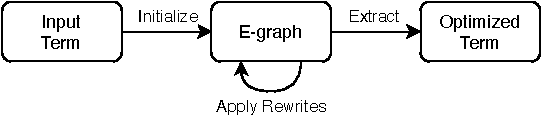
\includegraphics[width=0.9\linewidth]{eqsat}
  \end{minipage}
  \hfill
  \begin{minipage}{0.46\linewidth}
  \begin{lstlisting}[language=Python, gobble=4, numbers=left, basicstyle=\scriptsize\ttfamily]
    def equality_saturation(expr, rewrites):
      egraph = initial_egraph(expr)

      while not egraph.is_saturated_or_timeout():

        for rw in rewrites:
          for (subst, eclass) in egraph.ematch(rw.lhs):
            eclass2 = egraph.add(rw.rhs.subst(subst))
            egraph.merge(eclass, eclass2)

      return egraph.extract_best()
  \end{lstlisting}
  \end{minipage}
  \caption{
    等式饱和 的框图和伪代码。
    传统上,等式饱和 在整个算法中保持 \egraph 数据结构不变量。
  }
  \label{fig:eq-sat-bg}
\end{figure}


% \autoref{fig:eq-sat-bg} shows the equality saturation workflow.
% First, an initial \egraph is created from the input term.
% The core of the algorithm runs a set of rewrite rules until the \egraph is
%   saturated (or a timeout is reached).
% Finally, a procedure called \textit{extraction} selects the optimal represented
%   term according to some cost function.
% For simple cost functions, a bottom-up, greedy traversal of the \egraph suffices
%   to find the best term.
% Other extraction procedures have been explored for more complex cost
%   functions~\cite{spores, wu_siga19}.
\autoref{fig:eq-sat-bg} 展示了 等式饱和 工作流程。
首先,从输入的项创建初始 \egraph。
算法的核心运行一组重写规则,直到 \egraph 饱和或超时。
最后,称为 \textit{extraction(提取)} 的程序根据某些成本函数选择最优表示的项。
对于简单的成本函数,自底向上贪心遍历 \egraph 足以找到最佳项。
其他提取程序已经探索了更复杂的成本函数~\cite{spores, wu_siga19}。

% Equality saturation eliminates the tedious and often error-prone
%   task of choosing when to apply which rewrites,
% %Equality saturation turns a correctness problem into a performance problem,
%   promising an appealingly simple workflow: state the
%   relevant rewrites for the language, create an initial \egraph from a given
%   expression, fire the rules until saturation,
%   and finally extract the cheapest equivalent expression.
% Unfortunately, the technique remains ad hoc; prospective equality saturation
%   users must implement their own \egraphs customized to their language, avoid
%   performance pitfalls, and hack in the ability to do interpreted reasoning
%   that is not supported by purely syntactic rewrites.
% \egg aims to address each aspect of these difficulties.
等式饱和 消除了选择何时应用哪些重写的繁琐而容易出错的任务,
提供了一种简单易用的工作流程:确定语言相关重写,从给定表达式创建初始 \egraph ,运行规则直到饱和,
  最后提取最优的等价表达式。
不幸的是,这种技术仍然是特别定制的,
  等式饱和 用户必须自己实现专门针对语言的 \egraph,
  避免性能问题,并通过骇入(hack in)的方法实现纯语法重写无法支持的解释性推理。
\egg 旨在解决这些困难。

% \subsection{Equality Saturation and Theorem Proving}
\subsection{等式饱和 和 定理证明}

% An equality saturation engine and a theorem prover each have capabilities that
%   would be impractical to replicate in the other.
% Automated theorem provers like satisfiability modulo theory (SMT) solvers are
%   general tools that, in addition to supporting satisfiability queries,
%   incorporate sophisticated, domain-specific solvers to allow interpreted
%   reasoning within the supported theories.
% On the other hand, equality saturation is specialized for optimization, and its
%   extraction procedure directly produces an optimal term with respect to a given
%   cost function.
% % To replicate extraction with an SMT solver, one would have to resort to a more
% %   expensive enumerative approach.
等式饱和 引擎和定理验证器都有一些能力在对方身上复制是不切实际的。
像可满足模理论(SMT)求解器这样的自动化定理证明器是通用工具,
  除了支持可满足性查询外,还整合了专业的,领域特定的求解器,允许在支持的理论内进行解释性推理。
另一方面,等式饱和 是专门用于优化的,其提取过程直接产生关于给定成本函数的最优的项。

% \James{What enumerative approach? How do you know that one would "have to" resort to it?}

% While SMT solvers are indeed the more general tool,
%   equality saturation is not superseded by SMT;
%   the specialized approach can be much faster when the full generality of SMT is
%   not needed.
% To demonstrate this, we replicated a portion of the recent TASO paper~\cite{taso},
%   which optimizes deep learning models.
% As part of the work, they must verify a set of synthesized equalities with
%   respect to a trusted set of universally quantified axioms.
% TASO uses Z3~\cite{z3} to perform the
%   verification even though most of Z3's features
%   (disjunctions, backtracking, theories, etc.)
%   were not required.
% An equality saturation engine can also be used for verifying these equalities
%   by adding the left and right sides of
%   each equality to an \egraph,
%   running the axioms as rewrites,
%   and then checking if both sides end up in the same \eclass.
% Z3 takes 24.65 seconds to perform the verification;
%   \egg performs the same task in 1.56 seconds ($15\times$ faster),
%   or only 0.52 seconds ($47\times$ faster) when using
%   \egg's batched evaluation (\autoref{sec:egg-batched}).
尽管SMT求解器确实是更通用的工具,但 等式饱和 并不被 SMT 取代;
  当不需要 SMT 的完全通用性时,特异化的方法可能更快。
为了证明这一点,我们复制了最近 TASO 论文的一部分~\cite{taso},它优化了深度学习模型。
作为工作的一部分,他们必须验证一组合成等式,它们需要遵守一组具有普遍性的公理。 %?respect to 
TASO 使用 Z3~\cite{z3} 执行验证,即使大部分Z3的功能(或运算、回溯、理论等)都不需要使用。
等式饱和 也可以用于验证这些等式,
  将每个等式的左右两侧添加到 \egraph 中,将公理作为重写规则运行,
  然后检查两侧是否最终在同一个 \eclass 中。
Z3 花费 24.65 秒进行验证;\egg 在1.56秒(快 $15\times$)中完成相同任务,
  或在使用 \egg 的批量评估(\autoref{sec:egg-batched})时只需要 0.52 秒(快 $47\times$ )。
  
% --------------------

% \James{
  % The experimental/perf numbers in the last par of 2.4 feel out of place. Not sure how to fix...
% }

% However, their abilities overlap on a specific kind of theorem proving:
%   given a list of axioms in the form of universal quantified equalities,
%   prove two (or more) terms equal.
% Some SMT solvers support these kinds of queries, albeit in a limited fashion
%   since they are undecidable.
% \footnotetext{
%   Since these queries are undecidable, both SMT solvers and equality
%   saturation engines can either prove the inputs equal or fail to; they cannot
%   prove them unequal.
% }



%%% Local Variables:
%%% TeX-master: "egg"
%%% End:
